\documentclass[twoside,b5paper,10pt]{article}
\usepackage{AUTstyle}
\usepackage[english]{babel}
\usepackage{tabulary}
%\usepackage{biblatex}

\title{Comparison of text-unit extraction methods from bilingual corpus for predictive translation typing}
\author{Gabor Szabo \and Sandor Juhasz Dr.}

\institution{Department of Automation and Applied Informatics \\
Budapest University of Technology and Economics}

\email{harry.bme@gmail.com, Juhasz.Sandor@aut.bme.hu}

\headerTitle{Comparison of text-unit extraction\dots}
\headerAuthor{Gabor Szabo, Juhasz Sandor Dr.}

\newcommand{\itemdef}[2]{\item{\textbf{#1}: #2}}

%\addbibresource{predtyping.bib}

\begin{document}
\makeAutStyleTitle


\begin{abstract}
The goal of our research is to give predictive translation typing capabilities to computer-assisted translation tools. After summarizing the research in the field, including the TransType project, we present our dictionary based method, that uses simpler statistical techniques to extract possible text unit translations of a large, segmented, bilingual corpus. We investigated how using different types of text units (from words to multi-word n-grams; from strict word sequences to allow gaps in between) affects the size and the goodness of the resulting dictionary. For measuring size of the dictionary both entry number and physical size are considered, and for measuring goodness we chose the ratio of number of keystrokes saved by translators to the length of the translation. Measurements were carried out for the English-French language pair.
\end{abstract}


\begin{keywords}
predictive typing; 
statistical translation extraction; 
bilingual dictionary creation; 
text-unit collection; 
text-unit variants;
\end{keywords}

\section{Introduction}
\label{sec:Introdu}

Translators have a huge amount of work in today's fast and globalized world. Books, articles, news, essays and other kinds of written materials get published every day, and it is often required to have them translated into local languages. This amount of work cannot be successfully done without computer aid. Computer Assisted Translation (CAT) tools offer a variety of features to make translators' work more efficient. 

An interesting one of those features is auto-completion, or \emph{predictive translation typing}. Using that feature translators can save time and effort, and often spelling mistakes can be avoided. Numerous approaches have been designed for that since the mid-1990's. The main flow of research was applying techniques elaborated for traditional statistical machine translation with some tailoring. Church and Hovy suggested using machine translation (MT) for this purpose first, as an application for ``crummy'' machine translation \cite{church1993good}, because machine translation systems were not (and are not) able to produce high quality translation output without any human interaction.

Applying MT techniques turned out to be rewarding, as adapting them to the predictive scenario only required the addition of a prefix matching to the searching process, so the training methods could have been reused. However, machine translation engines are complex systems. This paper presents a much simpler, language independent approach. This method is also based on statistical processing, but instead of estimating and smoothing model parameters in iterations, it takes advantage of the large amount of memory available in state of the art computers to extract prediction information from bilingual corpora.

The rest of the paper is organized as follows: \sectionname~\ref{sec:rel-works} summarizes the related works in this field, then \sectionname~\ref{sec:dict-based} presents our approach of predictive translation typing. \sectionname~\ref{sec:meas} describes the measurements carried out, and \sectionname~\ref{sec:results} analyzes their results. \sectionname~\ref{sec:summary} summarizes the results and enumerates possible future works.


\section{Related works}
\label{sec:rel-works}

Predictive typing is widely used on devices with limited text input capabilities. It had an important role in speeding up text input on mobile phones with hard keys \cite{silfverberg2000predicting}, by allowing to press a key on the phone only once for each character. The system disambiguates using a dictionary, i.e. tries to determine which word the user wanted to type. How and Kan suggested using some context: automatic word completion was based on the keys pressed by the user and the previous word \cite{how2005optimizing}. Masui investigated the text-input productivity gain for English and Japanese language by using automatic word completion on pen-based soft key input devices, based on a predictive dictionary that stores words with their context \cite{masui1998efficient}. Approximate string matching based on spatial key layout was also presented in that work, to make the system tolerant for typos.

The groundbreaking research in predictive translation typing was the Trans\-Type project \cite{foster2002transtype}. Researchers of that project introduced the concept of using the production of the translation text as the key of interaction \cite{foster1997target}. That way the human translator ensures high-quality translation, while the computer can give a significant gain in productivity.

Machine translation engines designed in this project were based on IBM translation models \cite{brown1993mathematics}. In that paper five translation models were designed by IBM. Some of them were used in TransType, and some alternative translation models were designed (e.g. maximum entropy minimum divergence model \cite{foster2000maximum}), however, only words, or shorter sequence of words were offered as translation completion to the user.

Research were continued in the TransType2 project, a successor of TransType. Alternative translation models were designed, with the new approach to always give full sentence translation completion to the translator. In each iteration she accepts some prefix of the completion, then types some other text, and the computer gives another full sentence completion. Alignment templates, phrase-based models and stochastic finite-state transducers were examined in TransType2 as translation models \cite{barrachina2009statistical}.

The performance (in the sense of ``goodness'') of the systems designed were assessed by comparing translations produced by the system with a reference translation of a test parallel corpus. Some of the metrics measure the quality of the translation engine without any user activity, some of them try to estimate how much work can be saved by the translator using the system. The most frequently applied goodness metrics are the following:

\begin{itemize}
\itemdef{Bilingual evaluation understudy (BLEU)}{Based on how much of the reference translation text is produced (``covered'') by the translation system. Usually measured in \%. \cite{papineni2002bleu}}
\itemdef{Word error rate (WER)}{The Levenshtein-distance applied to the word strings produced by translation system and the reference translation (equals to the minimum number of substitution, insertion and deletion of words that is needed to transform the generated translation into the reference translation). It is normalized by the number of words in the reference sentences.}
\itemdef{Longest common subsequence}{The number of words in the longest common subsequence of words in the generated and reference translation, divided by the number of words in the reference translation. By subsequence a sequence of words are understood, that can be created by omitting some elements of the original sequence. I.e. subsequences may not be consecutive words in the original sequence.}
\itemdef{Keystroke ratio (KSR)}{Ratio of number of keystrokes to the total number of characters. Measured in \%.}
\end{itemize}

\section{Dictionary based translation prediction}
\label{sec:dict-based}

As mentioned in the introduction, machine translation engines are complex systems. This paper presents a simpler approach for predictive translation typing: it uses a dictionary to offer typing completions. In that sense, it is similar to the presented monolingual predictive typing solutions.

When prediction is based on the dictionary, the process is usually decoupled into two parts: a dictionary is created from some source once, and it is used to give predictions many times later. A bilingual dictionary is created and used in the presented case. The source of the dictionary is a large, segment-aligned, bilingual corpus. The corpus is processed with statistical methods in order to find translations of text fragments. 

Typing completions can be offered based on these text fragments: if a known text fragment is found in the source language sentence and the translator types something that is the beginning of a translation in the dictionary, then this known translation can be shown as a possible completion. Text fragments are called \emph{text units} in this paper. The exact definition of text unit is presented at the measurement's description, but they can be thought of like some words from a sentence that are linked together in a way, e.g. they form an expression or subsentence.

\begin{table}[hbt]
\caption{English-French parallel corpus for demonstration. Source: Proceedings of the European Parliament.}
\begin{center}
\begin{tabulary}{\textwidth}{|C|C|}
\hline
\textbf{English} & \textbf{French} \\
\hline
Madam President, the Presidency has already declared the result of the vote. & Madame la Pr�sidente, la pr�sidence a proclam� le r�sultat du vote. \\
\hline
There is no room for amendments. & Les modifications n'ont pas lieu d'�tre. \\
\hline
Madam President, in the earlier vote - and I will abide by your ruling on this matter - on the question of the strategic plan of the Commission I indicated that I would like to speak in advance of the vote on behalf of my Group. & Madame la Pr�sidente, lors du dernier vote � et je m'en remets � votre d�cision sur ce sujet - sur la question du plan strat�gique de la Commission, j'ai signal� que je demandais la parole avant le vote au nom de mon groupe. \\
\hline
\end{tabulary}
\end{center}
\label{tbl:sampleCorpus}
\end{table}

Dictionaries are created from a large, segment-aligned, bilingual corpus. An example corpus can be seen in \tablename~\ref{tbl:sampleCorpus}. The process includes four steps:
\begin{enumerate}
\item Count text unit occurrences separately for source and target language, and filter out rare ones. A text unit is considered rare if its occurrence is below a threshold denoted by $oc_{min}$.
\item For each remaining text unit of the source text, count the concomitant occurrences with each remaining text unit of the target text (i.e. how often they appear together in a segment and its translation).
\item For each source and target text unit pair, assign a score based on the individual and concomitant occurrences. If score falls under a given threshold $sc_{min}$, omit this pair.
\item Add the remaining $(source, target)$ text unit pairs to the resulting dictionary.
\end{enumerate}

In Step 1, filtering out rare text units helps avoid typographical errors and hapax legomena, and also helps to stay inside memory boundaries in Step 2. For Step 2, the input parallel corpus is processed again, this time handling the source segments with their aligned translation pair together. If a source text unit $s_i$ survived Step 1, and a target text unit $t_j$ survived Step 1, then an occurrence counter is increased for the $(s_i, t_j)$ pair. Multiple occurrences in a segment counts as one, both in Step 1 and Step 2. 

Each $(s, t)$ pair is assigned a score in Step 3, to decide if they are translations of each other (i.e. they should be in the dictionary). We used the \emph{Dice coefficient comparator} \cite{mcinnes2004extending} for scoring:
$$score = 2 \cdot \frac{N_{s,t}}{N_s + N_t}$$
Here $N_{s,t}$ denotes the number of sentence pairs where $s$ and $t$ occurs together, and $N_s$ and $N_t$ denotes the number of sentences where $s$ or $t$ occur, respectively. This score falls in the [0; 1] interval and expresses the ratio of concomitant occurrences to the sum of the individual occurrences.

In Step 4 a dictionary is built from the source language text units and its translations. An entry in the dictionary contains the source language text unit and a list of possible translations with the assigned scores. An example can be seen in \tablename~\ref{tbl:sampleDict}.

\begin{table}[hbt]
\caption{Sample English-French bilingual dictionary. Each English text unit is associated with a list of possible translations along their scores.}
\begin{tabular}{|c|c|}
\hline
\textbf{Source language text unit} & \textbf{List of possible translations} \\
\hline
I would & (je; 0.58), (voudrais; 0.44), (je voudrais; 0.31) \\
\hline
new & (nouvelle; 0.40) \\
\hline
Parliament & (Parlement; 0.89), (Parlement europ�en; 0.47) \\
\hline
and & (et; 0.89), (de; 0.64), \dots \\
\hline
\end{tabular}
\label{tbl:sampleDict}
\end{table}

\section{Measurements}
\label{sec:meas}

The goal of the measurement is to determine how different kinds of text units affect the ``goodness'' of the dictionary. Therefore, a fixed set of occurrence and score thresholds is used with each kind of text unit to create dictionaries, and the size and goodness of the dictionaries are measured. Size is measured both in physical size (e.g. in megabytes) and in entry number.

The metric for the goodness of the dictionary is keystroke ratio (KSR), as presented in \sectionname~\ref{sec:rel-works}. We chose this metric because it matches the effort needed from the translator when using the solution. It is automatically measured with a bilingual corpus. The source language sentences of the bilingual corpus are the sentences the hypothetical translator has to translate, and the target language sentences are the translations the translator would like to type. When the simulated translator starts translating a new sentence, the sentence is split into text units, and these text units are looked up in the dictionary for possible translations. If the translator starts typing a new word, and it is the prefix of some possible translations, those possible translations are offered as completions. The best six completions is shown to the translator, and she chooses the longest appropriate completion. The number of keystrokes saved by the translator is: $len(completion)-len(prefix)-index(completion)$. For sake of simplicity, ($100\% - KSR$) is displayed on the measurement results, as that is the ratio of the keystrokes \emph{saved} by the translator and using that figure greater values are better. 

The measurement presented in this paper uses these kinds of text unit: 
\begin{itemize}
\item only words
\item words and up to $n$-grams (separate measurements for $n = 3, 4, \dots, 7$)
\item all subsets of a 3-word sliding window.
\end{itemize}
Multiple word text units cannot overlap subsentence boundaries. 

The measurement program was written in C\# language targeting .NET Framework 4.5. Measurements were carried out on a 64-bit Microsoft Windows 8.1 operating system, using an Intel Core i7-2630QM 2.00 GHz CPU with 8 GB RAM.

The bilingual corpus were extracted from the proceedings of the European Parliament, downloaded from the OPUS project \cite{tiedemann2012parallel}. English-French language pair was chosen. 200k sentence pairs were used for dictionary creation and 20k for keystroke saving measurement. The thresholds used: $oc_{min} = 10^{-3}$, $sc_{min} = 3\cdot10^{-1}, 2.5\cdot10^{-1}, 2\cdot10^{-1}, 1.5\cdot10^{-1}, 10^{-1}, 5\cdot10^{-2}, 4\cdot10^{-2}, 3\cdot10^{-2}, 2\cdot10^{-2}, 1.5\cdot10^{-2}, 10^{-2}, 9\cdot10^{-3}, 8\cdot10^{-3}, 7\cdot10^{-3}, 6\cdot10^{-3}, 5.5\cdot10^{-3}, 5\cdot10^{-3}$. Thresholds were chosen so that dictionary size is between a few hundred kilobytes and a few hundred megabytes.

\begin{figure}[htb]
 \centerline{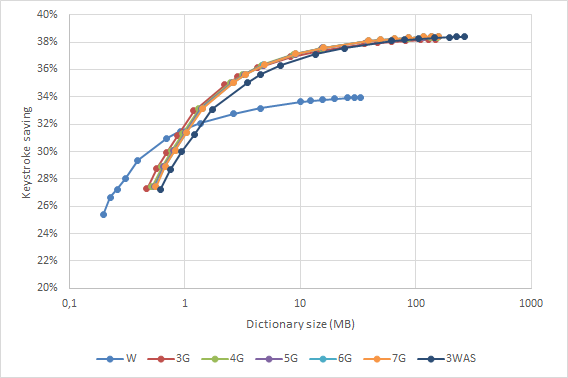
\includegraphics[width=.85\columnwidth]{.//Figure/fig_size.png}}
 \caption{Keystroke saving results based on the physical size of the dictionary. For small dictionary sizes the word-only approach is more efficient, but including $n$-grams result in greater keystroke saving beyond 1 megabyte.}
 \label{fig:bysize}
\end{figure}

\begin{figure}[hbt]
 \centerline{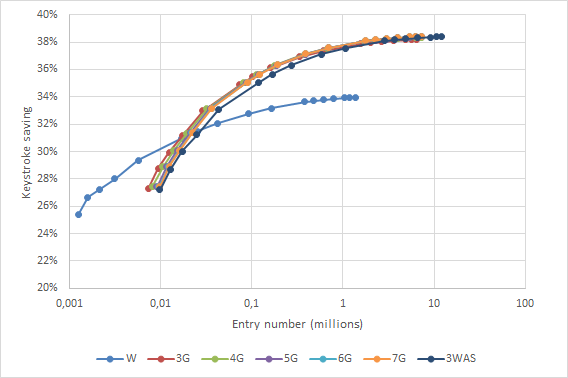
\includegraphics[width=.85\columnwidth]{.//Figure/fig_entrynum.png}}
 \caption{Keystroke saving results based on the entry number in the dictionary. For small dictionary sizes the word-only approach is more efficient, but including $n$-grams result in greater keystroke saving beyond 22 000 entries.}
 \label{fig:byentrynum}
\end{figure}

\begin{figure}[htb]
  \vspace{3pt}
  \centerline{
  \hbox{
  \hspace{0.0in}
        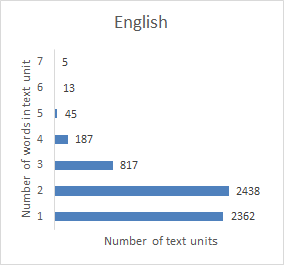
\includegraphics[width = 0.45\columnwidth]{Figure/fig_stat_en.png}
        \hspace{0.1\columnwidth}
        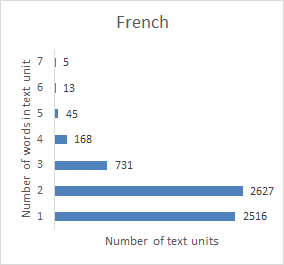
\includegraphics[width=0.45\columnwidth]{Figure/fig_stat_fr.png}
    }
  }
  \vspace{3pt}
  \hbox{\hspace{0.2\columnwidth} (a) \hspace{0.5\columnwidth} (b)}
  \caption{Distribution of word number in text units for the (a) English (b) French language, with 7-gram text unit collection method.}
  \label{fig:stats}
\end{figure}

\section{Results}
\label{sec:results}

Measurement results can be seen on \figurename~\ref{fig:bysize} and \figurename~\ref{fig:byentrynum}. The dictionary sizes on the horizontal axes are displayed with a logarithmic scale for better readability. The letters on the legend stands for: W -- words; ``$n$G'' -- up to $n$-grams; 3WAS -- all subsets of 3-word sliding window.

The shape of the curves and the relative positions are basically the same in the two figures. This means that both physical size and entry number can be used as basis for comparison, they give the same results.

Keystroke saving increases with dictionary size, but the marginal value of adding a new unit of size decreases, i.e. keystroke saving reaches a plateau. The maximum value is about 34\% for the only-word case and around 38.1--38.4\% for other cases.

Dictionaries built from $n$-grams have almost the same keystroke saving values. The maximum keystroke saving is 38.2\% for trigrams and 38.4\% for 7-grams. The difference is small. The reason behind this could be that only a few 4-5-6-7-grams pass the monolingual threshold $oc_{min}$ in Step 1 of dictionary creation. As it is shown on \figurename~\ref{fig:stats}(a) and \ref{fig:stats}(b), there are altogether 250 and 233 4-5-6-7-grams of the 5867 and 6105 text units for the English and French language respectively, which is around 4.3\% and 3.8\%. However, if we lower the $oc_{min}$ threshold, insufficient memory problems arise in the pairing and scoring step.

Similar insufficient memory problems occur when the dictionary is created from all subsets of a sliding window. It was manageable when the sliding window was 3 words wide, but the element number grows exponentially with the length of the sliding window. The ``all subsets of a 3-words wide sliding window'' method produced similar results as the $n$-grams, its values were between the values of 4-grams and 5-grams at higher sizes. 

Dictionaries using only words performs better at small sizes (the other curves seems to be shifted right in that interval), but including $n$-grams result in greater keystroke saving after 1 MB or 22k entries. Hence, using only words is better for small, compact dictionaries. On the other hand, state of the art computers can handle a 100 MB dictionary easily, so it's worth including longer text units in the dictionary.

\section{Summary}
\label{sec:summary}

A dictionary based approach for predictive translation typing was presented in this paper. We investigated one aspect of dictionary creation: how does different kinds of text units used during creation affect the dictionary size and the keystroke saving. Measurements were carried out on the English-French language pair.

It was stated that using multiple word text units in a dictionary makes its size bigger, but comes with greater keystroke saving. As state of the art computers can handle even the bigger dictionaries easily, the use of $n$-grams is advisable. Among them, using up to 3-grams makes the real difference compared to only words.

As future study, other kinds of text units could be investigated. The ``all subsets of an $n$-word sliding window'' version needs a sophisticated measure method to reduce memory consumption. Also, the order of the words in text units could be arbitrarily changed.

This dictionary based approach could be compared to monolingual prediction and to the TransType solutions. The sensitivity and optimal interval of the thresholds could also be measured, and different comparators could be used for scoring.


\section*{Acknowledgments}
 { \small The author would like to express his thanks to S�ndor Juh�sz Dr. for his support as a scientific advisor.
 }

\makeAutBib{predtyping}

\end{document}
